\documentclass[preprint]{revtex4-1}
\usepackage{graphicx}
\usepackage{epstopdf}
\usepackage{amsmath}
\usepackage{hyperref}
\usepackage{booktabs}
\usepackage{color}

\usepackage{SIunits}
\newcommand{\wstar}{-0.023}
\newcommand{\Qstar}{0.25}

\setlength{\tabcolsep}{10pt}

\newenvironment{sistema}%
  {\left\lbrace\begin{array}{@{}l@{}}}%
  {\end{array}\right.}


\usepackage{pgfplots}
\usepgfplotslibrary{external}
\usepgfplotslibrary{groupplots}
\tikzexternalize
\tikzset{external/force remake}
\tikzset{every mark/.append style={scale=0.8}}
\pgfplotsset{every axis/.append style={small}}

\begin{document}

\begin{figure}
	\centering
	\begin{tikzpicture}
		\begin{axis}[%
			anchor=right of south east,%
			width=0.45\textwidth, height=0.33\textwidth, %
			xlabel=$t/\tau_B$, xmode=log,%
			ylabel={Self ISF}, ymin=0,%
			legend columns=3, reverse legend, legend style={font=\tiny, at={(1,1.03)}, anchor=south east}, %
			%every mark/.append style={scale=0.5}%
			]
			\addplot file {LS3954.isf};
			\addplot file {LS4446.isf};
			\addplot file {LS4582.isf};
			\addplot file {LS5079.isf};
			\addplot file {go1.isf};
			\addlegendimage{legend image code/.code={\node[right] {$\phi\;\pm$};}};
			\legend{$0.497$, $0.535$, $0.540$, $0.555$, $0.575$, $0.003$};
			\node [anchor=south west] at (rel axis cs:0,0) {\bf a};
		\end{axis}
		\begin{axis}[%
			anchor=left of south west,%
			width=0.45\textwidth, %
			xlabel=$\phi$,%
			ylabel=$\tau_\alpha/\tau_B$, ymode=log, %
			ytick pos=right, ylabel near ticks,%
			]
			%\addplot+[mark=none, forget plot, domain=0.49:0.58] {0.7874243*exp(0.32826088*x/(0.60063652-x))};
			\addplot+[mark=none, forget plot, domain=0.49:0.58] {exp(0.28970401*x/(0.59841615-x))};
			\addplot+[only marks] table[x index=0, y index=1]{xi_phi.dat};
			\node at (rel axis cs:0,1) (a) {};
			\node [anchor=south west] at (rel axis cs:0,0) {\bf b};
		\end{axis}
		\begin{axis}[%
			tiny, at=(a), anchor=north west, %
			xlabel=$\phi$, xmin=0.49, xmax=0.58, xlabel near ticks,%
			ylabel=$\xi/\sigma$, ymin=0, ymax=4.5,%
			ytick pos=right, ylabel near ticks,%
			label style={font=\tiny}, %
			legend pos=north west,%
			axis background/.style={fill=white},%
			]
			\addplot+[mark=none, forget plot, domain=0.49:0.58] {0.41158778*((0.59773962-x)/0.59773962)^(-2.0/3.0)};
			\addplot+[only marks] table[x index=0, y index=2]{xi_phi.dat};
			\addplot+[mark=none, forget plot, domain=0.49:0.58] {0.18878182*((0.59773962-x)/0.59773962)^(-2.0/3.0)};
			\addplot+[only marks] table[x index=0, y index=3]{xi_phi.dat};
			\legend{$\xi_u$, $\xi_6$};
		\end{axis}
	\end{tikzpicture}
	\caption{Dynamics of the system. Self intermediate scattering function computed from the positions. Relaxation time $\tau_\alpha$ function of $\phi$. The line is the VFT fit. Inset: Dynamical and structural correlation length. Lines are power law fit.}
	\label{fig:vft}
\end{figure}

\begin{figure}
	\begin{tikzpicture}
		\pgfplotsset{
			extra tick style={grid=major},%
			every axis/.append style={%
				height=0.4\textwidth,
				ymin=0,ymax=0.6,%
				extra y ticks={\Qstar}, extra y tick labels={},%
				enlargelimits=false,axis on top,
				colormap={bw}{gray(0cm)=(1); gray(1cm)=(1); gray(10cm)=(0)},%
				colorbar sampled,%
				},%
		}
		\begin{groupplot}[
			group style={
				group size=2 by 1,%
				yticklabels at=edge left,%
				horizontal sep=0pt,%
				},%
			anchor=below south west,%
			width=0.45\textwidth,%
			xtick scale label code/.code={},%
			colorbar horizontal, colorbar style={%
				samples=6, xtick={ 0.20,0.4,0.6, 0.8},% 
				extra y ticks={},%
				/pgfplots/colorbar shift/.style={yshift=0.3cm},
				at={(parent axis.north)}, anchor=below south, width=0.9*\pgfkeysvalueof{/pgfplots/parent axis width},
				xticklabel pos=upper,%
				label style={font=\footnotesize},
				},%
			]
		\nextgroupplot[%
			ylabel={$Q_6$}, xlabel=$Q_4$,%
			xmin=0,xmax=0.22,%
			colorbar style={%
				xlabel={per units of $Q_4\cdot Q_6$},% 
				xticklabels={$10^{1}$, $10^{2}$, $10^{3}$, $10^{4}$},%
				},%
			xticklabel={$\pgfmathprintnumber[fixed,precision=2]{\tick}$}
			]
		\addplot graphics
		[xmin=0,xmax=0.2,ymin=0,ymax=0.6]
		{Q4Q6go1};
		\node [anchor=north west] at (rel axis cs:0,1) {\bf a};
		\node [below] at (axis cs:0.1909, 0.5745) {\textsc{fcc}};
		\node [below] at (axis cs:0.0972222, 0.484762) {\textsc{hcp}};
		\node [below] at (axis cs:0.0363696, 0.510688) {\textsc{bcc}};
		\draw[->, white,thick] (axis cs:0.05, 0.15) to [out=60, in=220] (axis cs:0.125, 0.4);
		
		\nextgroupplot[%
			xlabel=$10^3 \cdot w_4$, %
			xmin=-0.002,xmax=0.002,%
			xtickmin=-0.0015,%
			extra x ticks=0, extra x tick labels={},
			colorbar style={%
				xlabel={per units of $w_4\cdot Q_6$},% 
				xticklabels={$10^{3}$, $10^{4}$, $10^{5}$, $10^{6}$},%
				},%
			]
		\addplot graphics
		[xmin=-0.002,xmax=0.002,ymin=0,ymax=0.6]
		{w4Q6go1};
		\node [anchor=north west] at (rel axis cs:0,1) {\bf b};
		\node [below] at (axis cs:-0.00067221, 0.5745) {\textsc{fcc}};
		\node [below] at (axis cs:7.47E-05, 0.484762) {\textsc{hcp}};
		%\node [below] at (axis cs:-0.01274716, 0.510688) {\textsc{bcc}};
		\node [above] at (axis cs:0.0015, \Qstar) {\footnotesize{$Q_6^*$}};
		\draw[->, white,thick] (axis cs:0, 0.15) to [out=120, in=280] (axis cs:-0.0005, 0.4);
		\draw[->, white,thick] (axis cs:0, 0.15) to (axis cs:7E-05, 0.35);
		
		\end{groupplot}
		
		\begin{groupplot}[
			group style={
				group size=2 by 1,%
				yticklabels at=edge left,%
				horizontal sep=0pt,%
				},%
			anchor=above north west,%
			width=0.38\textwidth,%
			xlabel=$10^2 \cdot w_6$,%
			xmin=-0.052,xmax=0.01,%
			extra x ticks={\wstar, -0.00782},%
			extra x tick labels={,},%
			xtick scale label code/.code={},%
			colorbar right, colorbar style={%
				samples=6, ytick={ 0.20,0.4,0.6, 0.8},% 
				yticklabels={$10^{1}$, $10^{2}$, $10^{3}$, $10^{4}$},%
				ylabel={per units of $w_6\cdot Q_6$},%
				extra x ticks={},%
				extra y ticks={},%
				label style={font=\footnotesize},
				},%
			]
		
		\nextgroupplot[ylabel={$Q_6$}, xtickmax=0,]
		\addplot graphics
		[xmin=-0.052,xmax=0.052,ymin=0,ymax=0.6]
		{u6Q6go1_scale};
		\node [anchor=north west] at (rel axis cs:0,1) {\bf c};
		\node at (axis cs:\wstar,0.6) (a) {};
		\node at (axis cs:-0.00782,0.6) (b) {};
		\node [below] at (axis cs:-0.0026, 0.5745) {\textsc{fcc}};
		\node [below, right] at (axis cs:-0.052, 0.05) {\textsc{Ico}};
		\draw[->, white,thick] (axis cs:-0.001, 0.15) to [out=90, in=275] (axis cs:-0.0015, 0.33);
		\draw[->, white,thick] (axis cs:-0.001, 0.15) to [out=180, in=30] (axis cs:-0.025, 0.12);
		
		\nextgroupplot
		\addplot graphics
		[xmin=-0.052,xmax=0.052,ymin=0,ymax=0.6]
		{u6Q6phi3954_scale};
		\node [anchor=north west] at (rel axis cs:0,1) {\bf d};
		\node [above] at (axis cs:-0.04, \Qstar) {\footnotesize{$Q_6^*$}};
		%\node [anchor=north east] at (rel axis cs:1, 1) {\footnotesize{$\phi = 0.497 \pm 0.03$}};
		\node [left] at (axis cs:\wstar,0.4) {\footnotesize $w_6^*$};
		\node [right] at (axis cs:-0.00782,0.4) {\footnotesize $w_6^{dod}$};
		
		\end{groupplot}
	\end{tikzpicture}
	\caption{Population of local structures function of \textsc{boo}. (a-c) For our deepest supercooled sample ($\phi=0.575\pm 0.03$) in the $(Q_4,Q_6)$-plane (a), $(w_4,Q_6)$-plane (b) and $(w_6,Q_6)$-plane (c). (d) is the same as (c) but for a liquid near the freezing point ($\phi = 0.497 \pm 0.03$). Colour represent the probability to find the structure (log scale). The arrows stress the ordering tendencies: the tendency toward \textsc{fcc} is always visible, but a tendency toward \textsc{hcp} can be distinguished in (b) and the tendency toward icosahedral order is visible in (c).}
	\label{fig:maps}
\end{figure}


\begin{figure}
	\begin{tikzpicture}
		\begin{axis}[%
			anchor=below south,%
			width=0.5\textwidth,%
			height=0.5\textwidth,%
			ylabel=$Q_6$,%
			ymin=0,ymax=0.6,%
			xlabel=$10^2 \cdot w_6$,%
			xmin=-0.052,xmax=0.01,%
			xtick scale label code/.code={},%
			enlargelimits=false,axis on top,
			colormap={sd}{color(0cm)=(black) rgb(1cm)=(0.5, 0, 0) rgb(2cm)=(1, 0.5, 0) color(3cm)=(yellow) rgb(4cm)=(0.5, 0.75, 1) rgb(5cm)=(0.5, 0.75, 1)},%
			extra x ticks={\wstar, -0.00782},%
			extra x tick style={grid=major,	tick label style={anchor=south west}},%
			extra x tick labels={,},%
			extra x tick style={grid=major},
			extra y ticks={\Qstar},
			extra y tick style={grid=major},
			extra y tick labels={},%
			colorbar sampled, colorbar style={%
				samples=5, ytick={ 0, 0.25, 0.5, 0.75},% 
				yticklabels={$0$, $0.5$, $1$, $1.5$},%
				ylabel=${\mathcal{P}r(t^{dh})}/{\langle\Delta r^2(t^{dh}) \rangle}$,%
				extra x ticks={},%
				yticklabel pos=right,%
				label style={font=\footnotesize},
				},%
			]
			\addplot graphics [xmin=-0.052,xmax=0.052,ymin=0,ymax=0.6]{sd_u6Q6_go1_color};
			\node [anchor=north west] at (rel axis cs:0,1) {\bf a};
			\node [above] at (axis cs:-0.04, \Qstar) {\footnotesize{$Q_6^*$}};
			\node [anchor=west] at (rel axis cs:0, 0.8) {\footnotesize{$\phi = 0.575 \pm 0.03$}};
			\node [left] at (axis cs:\wstar,0.55) {\footnotesize $w_6^*$};
			\node [left] at (axis cs:-0.00782,0.55) {\footnotesize $w_6^{dod}$};
			\node [below] at (axis cs:-0.0026, 0.5745) {\textsc{fcc}};
			\node [below, right] at (axis cs:-0.052, 0.05) {\textsc{Ico}};
		\end{axis}
		\pgfplotsset{every axis plot/.append style={only marks}}
		\begin{groupplot}[%
			group style={
				group size=2 by 2,%
				yticklabels at=edge left,%
				horizontal sep=0pt,%
				},%
			anchor=outer north east,%
			width=0.5\textwidth,%
			ymin=0, ymax=1.5,%
			extra x tick style={grid=major,	tick label style={anchor=south west}},%
			extra y ticks={1},%
			extra y tick style={grid=major,	tick label style={anchor=south west}}, extra y tick labels={},%
			%legend columns=5,%
			legend style={
				font=\footnotesize,
				%at={(1,1)}, anchor=south,%
				at={(1,1)}, anchor=north east
				},%
			]
			\nextgroupplot[%
				xlabel=$10^2 \cdot w_6$, xmin=-0.0521089193, xmax=0.01,%
				xtickmax={0},%
				xtick scale label code/.code={},%
				ylabel=${\mathcal{P}r(t^{dh})}/{\langle\Delta r^2(t^{dh}) \rangle}$,
				extra x ticks={\wstar, -0.00782}, extra x tick labels={$w_6^*$,$w_6^{dod}$},%
				extra y tick labels={bulk}
				]
			
			%\addplot table[x index=0, y expr={\thisrowno{1}/\thisrowno{2}}]{sd_nb_u6_phi3954.txt};
			\addplot table[x index=0, y expr={\thisrowno{1}/\thisrowno{2}}]{sd_nb_u6_phi4446.txt};
			\addplot table[x index=0, y expr={\thisrowno{1}/\thisrowno{2}}]{sd_nb_u6_phi5079.txt};
			\addplot table[x index=0, y expr={\thisrowno{1}/\thisrowno{2}}]{sd_nb_u6_go1.txt};
			\addplot+[domain=-0.0521089193:0.01, sharp plot, no markers] {9.34701 * x + 1.03764};
			\draw[->, thick] (rel axis cs:0.2, 0.9) to (rel axis cs:0, 0.9);
			\node[right] at (rel axis cs:0.2, 0.9) {\footnotesize Icosahedron};
			\node [anchor=south west] at (rel axis cs:0,0) {\bf b};
			
			\nextgroupplot[%
				xlabel=$Q_6$, xmin=0, xmax=0.5745,%
				extra x ticks={\Qstar}, extra x tick labels={$Q_6^*$},%				
				]
			\addlegendimage{legend image code/.code={\node[right] {$\phi\;\pm$};}};
			\legend{$0.003$,%$0.497$, 
				$0.535$, $0.555$, $0.575$};
			%\addplot table[x index=0, y expr={\thisrowno{1}/\thisrowno{2}}]{sd_nb_Q6_3954.txt};
			\addplot table[x index=0, y expr={\thisrowno{1}/\thisrowno{2}}]{sd_nb_Q6_4446.txt};
			\addplot table[x index=0, y expr={\thisrowno{1}/\thisrowno{2}}]{sd_nb_Q6_5079.txt};
			\addplot table[x index=0, y expr={\thisrowno{1}/\thisrowno{2}}]{sd_nb_Q6_go1.txt};
			\draw[->, thick] (rel axis cs:0.8, 0.45) to (rel axis cs:1, 0.45);
			\node[left] at (rel axis cs:0.8, 0.45) {\footnotesize \textsc{fcc}};
			\node [anchor=south west] at (rel axis cs:0,0) {\bf c};
		\end{groupplot}
	\end{tikzpicture}
	\caption{{\bf Bond order propensity.} (a) Normalised propensity in the $(w_6, Q_6)$-plane for our most deeply supercooled sample. The colour scale is saturated at $1.5$ times the bulk mean square displacement. (b-c) Normalised propensity for icosahedral and crystalline order parameters respectively. Bulk mean square displacement is at 1. Perfect structures are on the edge of each plot. The line is a guide for the eye stressing the collapse of the $w_6$-propensity at all volume fractions.}
	\label{fig:msd_Q6_w6}
\end{figure}


\begin{figure}
	\centering
	\begin{tikzpicture}[lab/.style={right, inner sep=0.05em, fill=white, font=\footnotesize}]
	\node[anchor=west, draw, inner sep=0, outer xsep=0.5em] (all) {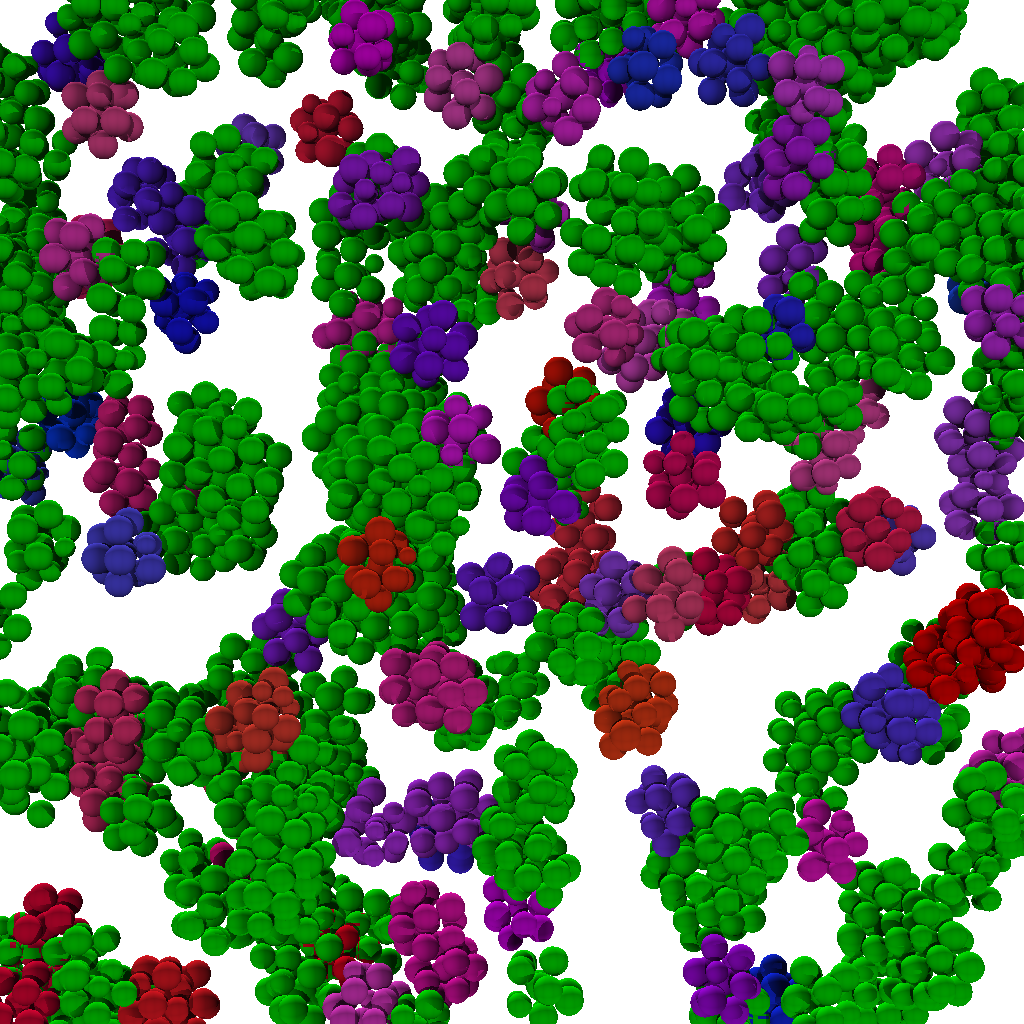
\includegraphics[width=0.75\textwidth]{mrco_ico_scale_go1-0023.png}};
	\matrix[%
		matrix anchor=east, draw, font=\footnotesize,% 
		column 1/.style={text height=0.8em, text depth=0.2em},%
		column 2/.style={circle, shade, inner sep=0.01\textwidth},%
		] (l)
	{
		\node{Icosahedra}; & \node[ball color=red!33!blue] (b2) {}; \\
		\node{Crystal-like}; & \node[ball color=green!66!black] {}; \\
	};
	\node[above] at (l.north) (ico) {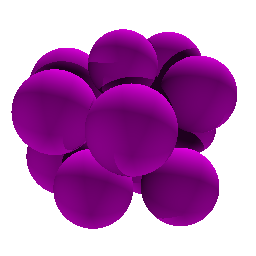
\includegraphics[width=0.2\textwidth]{one_ico.png}};
	\node at (ico.north){$w_6=w_6^*$};
	\node[below] at (l.south) (mrco) {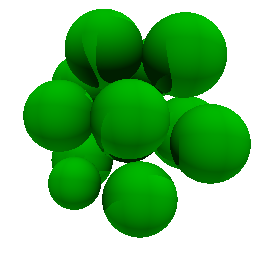
\includegraphics[width=0.2\textwidth]{one_mrco.png}};
	\node at (mrco.south) {$Q_6=Q_6^*$};
	\node[lab, anchor=north] at (all.north) {$\phi=0.575$};
	\end{tikzpicture}
	\caption{Computer reconstruction from confocal microscopy coordinates of a typical configuration in our most deeply supercooled sample. Depth is $\sim 12\sigma$. Only ordered particles and their neighbours are displayed. Each particle is plotted with its real radius. Two icosahedral particle are shown in the same shade if they belong to the same cluster. If a particle is neighbouring both kind of structures, it is displayed as icosahedral. Left: Example of structures at the respective threshold values: distorted icosahedron (top) and crystal-like cluster (bottom).}
	\label{fig:3D}
\end{figure}

\end{document}